\documentclass[10pt]{article}

\usepackage[a4paper, margin=2cm]{geometry}
\usepackage[T1]{fontenc}
\usepackage[utf8]{inputenc}
\usepackage[scaled=0.85]{beramono}  % bold tt
\renewcommand{\familydefault}{\ttdefault}
\setlength{\parindent}{0cm}

\usepackage[english]{babel}
\usepackage{graphicx}
\usepackage[hidelinks]{hyperref}
\usepackage{xcolor}
\definecolor{dark-blue}{rgb}{0.15,0.15,0.4}
\hypersetup{colorlinks, linkcolor={dark-blue}, citecolor={dark-blue}, urlcolor={dark-blue}}

\usepackage{lastpage}
\usepackage{fancyhdr}
\pagestyle{fancy}
\renewcommand{\headrulewidth}{0pt}
\cfoot{Page \thepage\ of \pageref{LastPage}}

\usepackage{tikz}
\usetikzlibrary{tikzmark, calc}

\newcommand{\caixa}[1]{\bigskip\tikzmark{#1}%
\raisebox{-0.8mm}{
\begin{tikzpicture}
\draw[thick] (0,0) rectangle (0.35,0.35);
\draw[thick] (0.1,0.175) -- (0.25,0.175);
\end{tikzpicture}}}


\begin{document}

% photo and personal information
\begin{minipage}{0.12\linewidth}
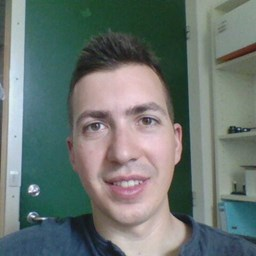
\includegraphics[width=\linewidth]{imgs/photo}
\end{minipage}
\begin{minipage}{0.88\linewidth}
\textbf{\large Ricardo Pereira de Magalhães Cruz}\\
\raisebox{-0.25\height}{
\includegraphics[width=1em]{imgs/email}} \href{mailto:ricardo.pdm.cruz@gmail.com}{ricardo.pdm.cruz@gmail.com}\\
\raisebox{-0.25\height}{
\includegraphics[width=1em]{imgs/www}} \href{https://rpmcruz.github.io}{https://rpmcruz.github.io}\\
(+351)934741617 $\bullet$ Valongo, Portugal
\end{minipage}

\bigskip
\textcolor{black!80}{\colorbox{black!10}{\begin{minipage}{\linewidth}
For the last five years, I have been working as a machine learning researcher at INESC TEC. I have just finished my Ph.D. thesis which I will defend very soon. Meanwhile, I also have been helping at FEUP as a teacher assistant: teaching Python and C++.
As a machine learning researcher, I have worked mostly on deep learning applied to computer vision, using both TensorFlow and PyTorch. In the past, I have participated in many open-source projects and also did much consulting work: on web development (flask), databases (mongo, postgres), multimedia (sdl, gtk, qt), server administration (hpc) and others.
In terms of education, I am about to finish my Ph.D. in computer science. I have a masters in applied mathematics and a bachelors in computer science.
\end{minipage}}}

%%%%%%%%%%%%%%%%%%%%%%%%%%%%%%%%%%%%%%%%%%%%%%%%%%%%%%%%

\filbreak
\caixa{education} Education

\bigskip
\begin{tabular}{p{1mm}lp{46em}}
& \tikzmark{e1}\textbf{ (2021) } & PhD in Computer Science (currently waiting for defense!)  \\
& & \textcolor{black!60}{ co-joint University of Porto, Minho and Aveiro } \\
& \tikzmark{e2}\textbf{ 2015 } & MSc in Applied Mathematics (Grade=18/20) \\
& & \textcolor{black!60}{ Faculty of Sciences, University of Porto } \\
& \tikzmark{e3}\textbf{ 2012 } & BSc in Computer Science (Grade=16/20) \\
& & \textcolor{black!60}{ Faculty of Sciences, University of Porto } \\
\end{tabular}

\begin{tikzpicture}[remember picture, overlay]
\draw[dashed] let \p1=(pic cs:e1) in ({2mm,\y1+1mm}) -- ++ (4mm,0);
\draw[dashed] let \p1=(pic cs:e2) in ({2mm,\y1+1mm}) -- ++ (4mm,0);
\draw[dashed] let \p1=(pic cs:e3) in ({2mm,\y1+1mm}) -- ++ (4mm,0);
\draw[dashed] let \p1=(pic cs:education), \p2=(pic cs:e3) in ({2mm,\y1-1mm}) -- ({2mm,\y2+1mm});
\end{tikzpicture}

%%%%%%%%%%%%%%%%%%%%%%%%%%%%%%%%%%%%%%%%%%%%%%%%%%%%%%%%

\filbreak
\caixa{career} Career

\bigskip
\begin{tabular}{p{1mm}lp{46em}}
& \tikzmark{c1}\textbf{ 2018--2021 } & Teacher Assistant (Python and C/C++) \\
& & \textcolor{black!60}{ Faculty of Engineering, University of Porto } \\
& \tikzmark{c2}\textbf{ 2016--2020 } & PhD Grant (deep learning and computer vision) \\
& & \textcolor{black!60}{ INESC TEC } \\
& \tikzmark{c3}\textbf{ 2015 } & Research Grant (machine learning) \\
& & \textcolor{black!60}{ INESC TEC } \\
& \tikzmark{c4}\textbf{ 2014 } & Research Grant (epidemiology modelling) \\
& & \textcolor{black!60}{ Mathematics Center of the University of Porto } \\
& \tikzmark{c5}\textbf{ 2007 } & Google Grant: Summer of Code (dynamic layouts) \\
& & \textcolor{black!60}{ OpenOffice.org } \\
& \tikzmark{c6}\textbf{ 2006 } & Google Grant: Summer of Code (YaST GTK port) \\
& & \textcolor{black!60}{ Novell / openSUSE } \\
\end{tabular}

\begin{tikzpicture}[remember picture, overlay]
\draw[dashed] let \p1=(pic cs:c1) in ({2mm,\y1+1mm}) -- ++ (4mm,0);
\draw[dashed] let \p1=(pic cs:c2) in ({2mm,\y1+1mm}) -- ++ (4mm,0);
\draw[dashed] let \p1=(pic cs:c3) in ({2mm,\y1+1mm}) -- ++ (4mm,0);
\draw[dashed] let \p1=(pic cs:c4) in ({2mm,\y1+1mm}) -- ++ (4mm,0);
\draw[dashed] let \p1=(pic cs:c5) in ({2mm,\y1+1mm}) -- ++ (4mm,0);
\draw[dashed] let \p1=(pic cs:c6) in ({2mm,\y1+1mm}) -- ++ (4mm,0);
\draw[dashed] let \p1=(pic cs:career), \p2=(pic cs:c6) in ({2mm,\y1-1mm}) -- ({2mm,\y2+1mm});
\end{tikzpicture}

%%%%%%%%%%%%%%%%%%%%%%%%%%%%%%%%%%%%%%%%%%%%%%%%%%%%%%%%

\filbreak
\caixa{others} Other related work

\bigskip
\begin{tabular}{p{1mm}lp{46em}}
& \tikzmark{o1}\textbf{ 2018-2020 } & Consulting for a geography team at FLUP \\
& & \textcolor{black!60}{ In total, I have done seven scraping and automation jobs. } \\
& \tikzmark{o2}\textbf{ 2018-2019 } & Mentor at Coursera \\
& & \textcolor{black!60}{ Andrew Ng's course on Improving Deep Neural Networks: Hyperparameter tuning, Regularization and Optimization } \\
& \tikzmark{o3}\textbf{ 2014 } & Consulting at Flykt \\
& & \textcolor{black!60}{ Search algorithms for travel destinations. } \\
\end{tabular}

\begin{tikzpicture}[remember picture, overlay]
\draw[dashed] let \p1=(pic cs:o1) in ({2mm,\y1+1mm}) -- ++ (4mm,0);
\draw[dashed] let \p1=(pic cs:o2) in ({2mm,\y1+1mm}) -- ++ (4mm,0);
\draw[dashed] let \p1=(pic cs:o3) in ({2mm,\y1+1mm}) -- ++ (4mm,0);
\draw[dashed] let \p1=(pic cs:others), \p2=(pic cs:o3) in ({2mm,\y1-1mm}) -- ({2mm,\y2+1mm});
\end{tikzpicture}

%%%%%%%%%%%%%%%%%%%%%%%%%%%%%%%%%%%%%%%%%%%%%%%%%%%%%%%%

\filbreak
\caixa{awards} Awards

\bigskip
\begin{tabular}{p{1mm}lp{46em}}
& \tikzmark{a1}\textbf{ 2020 } & Best Oral Presentation: Training Convolutional Neural Networks to be Background Invariant \\
& & \textcolor{black!60}{ RECPAD 2020 conference } \\
& \tikzmark{a2}\textbf{ 2021 } & Pedagogical Recognition Award \\
& & \textcolor{black!60}{ Faculty of Engineering, University of Porto } \\
& \tikzmark{a3}\textbf{ 2021 } & Sustainable Ideas \\
& & \textcolor{black!60}{ Faculty of Engineering, University of Porto } \\
\end{tabular}

\begin{tikzpicture}[remember picture, overlay]
\draw[dashed] let \p1=(pic cs:a1) in ({2mm,\y1+1mm}) -- ++ (4mm,0);
\draw[dashed] let \p1=(pic cs:a2) in ({2mm,\y1+1mm}) -- ++ (4mm,0);
\draw[dashed] let \p1=(pic cs:a3) in ({2mm,\y1+1mm}) -- ++ (4mm,0);
\draw[dashed] let \p1=(pic cs:awards), \p2=(pic cs:a3) in ({2mm,\y1-1mm}) -- ({2mm,\y2+1mm});
\end{tikzpicture}

%%%%%%%%%%%%%%%%%%%%%%%%%%%%%%%%%%%%%%%%%%%%%%%%%%%%%%%%

\filbreak
\caixa{publications} Publications

\bigskip
\begin{tabular}{p{1mm}lp{46em}}
& \tikzmark{p1}\textbf{ 2021 } & Ordinal Losses for Classification of Cervical Cancer Risk [accepted] \\
& & \textcolor{black!60}{ T. Albuquerque, R. Cruz, J. Cardoso } \\
& & \textcolor{black!60}{ PeerJ Computer Science } \\
& \tikzmark{p2}\textbf{ 2021 } & Background Invariance by Adversarial Learning [accepted] \\
& & \textcolor{black!60}{ R. Cruz, R. Prates, E. Filho, J. Costa, J. Cardoso } \\
& & \textcolor{black!60}{ 25th International Conference on Pattern Recognition (ICPR), IEEE } \\
& \tikzmark{p3}\textbf{ 2019 } & Automatic Augmentation by Hill Climbing \\
& & \textcolor{black!60}{ R. Cruz, J. Costa, J. Cardoso } \\
& & \textcolor{black!60}{ 28th International Conference on Artificial Neural Networks (ICANN), Springer } \\
& \tikzmark{p4}\textbf{ 2019 } & Averse Deep Semantic Segmentation \\
& & \textcolor{black!60}{ R. Cruz, J. Costa, J. Cardoso } \\
& & \textcolor{black!60}{ 41st Engineering in Medicine and Biology Conference (EMBC), IEEE } \\
& \tikzmark{p5}\textbf{ 2019 } & Insulator visual non-conformity detection in overhead power distribution lines using deep learning \\
& & \textcolor{black!60}{ R. Prates, R. Cruz, A. Marotta, R. Ramos, E. Filho, J. Cardoso } \\
& & \textcolor{black!60}{ Journal Computers \& Electrical Engineering, Springer } \\
& \tikzmark{p6}\textbf{ 2018 } & A Class Imbalance Ordinal Method for Alzheimer’s Disease Classification \\
& & \textcolor{black!60}{ R. Cruz, M. Silveira, J. Cardoso } \\
& & \textcolor{black!60}{ 2018 International Workshop on Pattern Recognition in Neuroimaging (PRNI), IEEE } \\
& \tikzmark{p7}\textbf{ 2018 } & Binary ranking for ordinal class imbalance \\
& & \textcolor{black!60}{ R. Cruz, K. Fernandes, J. Costa, M. Pérez Ortiz, J. Cardoso } \\
& & \textcolor{black!60}{ Journal Pattern Analysis and Applications, Springer } \\
& \tikzmark{p8}\textbf{ 2018 } & Deep image segmentation by quality inference \\
& & \textcolor{black!60}{ K. Fernandes, R. Cruz, J. Cardoso } \\
& & \textcolor{black!60}{ International Joint Conference on Neural Networks (IJCNN), IEEE } \\
& \tikzmark{p9}\textbf{ 2017 } & Constraining type II error: building intentionally biased classifiers \\
& & \textcolor{black!60}{ R. Cruz, K. Fernandes, J. Costa, J. Cardoso } \\
& & \textcolor{black!60}{ International Work-conference on Artificial Neural Networks (IWANN), Springer } \\
& \tikzmark{p10}\textbf{ 2017 } & Fine-to-coarse ranking in ordinal and imbalanced domains: an application to liver transplantation \\
& & \textcolor{black!60}{ M. Pérez-Ortiz, K. Fernandes, R. Cruz, J. Cardoso } \\
& & \textcolor{black!60}{ International Work-conference on Artificial Neural Networks (IWANN), Springer } \\
& \tikzmark{p11}\textbf{ 2017 } & Combining ranking with traditional methods for ordinal class imbalance \\
& & \textcolor{black!60}{ R. Cruz, K. Fernandes, J. Costa, M. Pérez-Ortiz, J. Cardoso } \\
& & \textcolor{black!60}{ International Work-conference on Artificial Neural Networks (IWANN), Springer } \\
& \tikzmark{p12}\textbf{ 2017 } & Ordinal class imbalance with ranking \\
& & \textcolor{black!60}{ R. Cruz, K. Fernandes, J. Costa, M. Pérez-Ortiz, J. Cardoso } \\
& & \textcolor{black!60}{ Iberian conference on pattern recognition and image analysis (Ibpria), Springer } \\
& \tikzmark{p13}\textbf{ 2016 } & Tackling class imbalance with ranking \\
& & \textcolor{black!60}{ R. Cruz, K. Fernandes, J. Costa, J. Cardoso } \\
& & \textcolor{black!60}{ International Joint Conference on Neural Networks (IJCNN), IEEE } \\
\end{tabular}

\begin{tikzpicture}[remember picture, overlay]
\draw[dashed] let \p1=(pic cs:p1) in ({2mm,\y1+1mm}) -- ++ (4mm,0);
\draw[dashed] let \p1=(pic cs:p2) in ({2mm,\y1+1mm}) -- ++ (4mm,0);
\draw[dashed] let \p1=(pic cs:p3) in ({2mm,\y1+1mm}) -- ++ (4mm,0);
\draw[dashed] let \p1=(pic cs:p4) in ({2mm,\y1+1mm}) -- ++ (4mm,0);
\draw[dashed] let \p1=(pic cs:p5) in ({2mm,\y1+1mm}) -- ++ (4mm,0);
\draw[dashed] let \p1=(pic cs:p6) in ({2mm,\y1+1mm}) -- ++ (4mm,0);
\draw[dashed] let \p1=(pic cs:p7) in ({2mm,\y1+1mm}) -- ++ (4mm,0);
\draw[dashed] let \p1=(pic cs:p8) in ({2mm,\y1+1mm}) -- ++ (4mm,0);
\draw[dashed] let \p1=(pic cs:p9) in ({2mm,\y1+1mm}) -- ++ (4mm,0);
\draw[dashed] let \p1=(pic cs:p10) in ({2mm,\y1+1mm}) -- ++ (4mm,0);
\draw[dashed] let \p1=(pic cs:p11) in ({2mm,\y1+1mm}) -- ++ (4mm,0);
\draw[dashed] let \p1=(pic cs:p12) in ({2mm,\y1+1mm}) -- ++ (4mm,0);
\draw[dashed] let \p1=(pic cs:p13) in ({2mm,\y1+1mm}) -- ++ (4mm,0);
\draw[dashed] let \p1=(pic cs:publications), \p2=(pic cs:p13) in ({2mm,\y1-1mm}) -- ({2mm,\y2+1mm});
\end{tikzpicture}

\bigskip
\textcolor{black!80}{\colorbox{black!10}{\begin{minipage}{\linewidth}
Recommendation contacts will be provided upon request.\\
Consult my github for more projects: \url{https://github.com/rpmcruz}.
\end{minipage}}}


\end{document}
